\documentclass[aspectratio=169]{beamer}
\usepackage{framed}
\usepackage{lhps}

\renewcommand{\ImageSource}{L2-Images/}
\begin{document}

\section{Причинно-следственное мышление}

\begin{bframe}
\begin{Reason}
	\from{Если идет дождь, то земля становится мокрой}
	\from{Идет дождь}
	\conc{Земля мокрая}
\end{Reason}
\end{bframe}

\begin{bframe}
\begin{Reason}
	\from[3]{Если идет дождь, то капли воды находятся в воздухе}
	\from[3]{Если капли воды находятся в воздухе, то они падают на землю}
	\from[3]{Если много капель воды падает на землю, то земля смешивается с водой}
	\from[3]{Если земля смешивается с водой, то земля становится мокрой}
	\conc[2-]{Если идет дождь, то земля становится мокрой}
	\from[1]{Если идет дождь, то земля становится мокрой}
	\from[1-]{Идет дождь}
	\conc[1-]{Земля мокрая}
\end{Reason}
\end{bframe}

\begin{bframe}
\begin{Reason}
	\from[7-]{Если тело тяжелее воздуха, то оно падает на землю}
	\conc[6-]{\bf Ну, существуют силы гравитации...}
	\from[5]{\bf Ну, существуют силы гравитации...}
	\conc[4-]{Если тело тяжелее воздуха, то оно падает на землю}
	\from[3]{Если тело тяжелее воздуха, то оно падает на землю}
	\from[3-]{Капли воды тяжелее воздуха}
	\conc[2-]{Если капли воды находятся в воздухе, то они падают на землю}
	\from[1]{Если капли воды находятся в воздухе, то они падают на землю}
\end{Reason}
\end{bframe}

\begin{bframe}
\begin{Reason}
\from[3-]{Валерьана содержит актинидин}
\from[3-]{Актинидин имеет запах, схожий с  3-меркапто-3-метилбутан-1-ола}
\from[3-]{3-меркапто-3-метилбутан-1-ол содержится в моче кошачьих}
\from[4]{\bf Ну, наверное, это вещество как-то особенно действует на нервную систему...}
\conc[2-]{Если коту дать валерьану, он начнет вести себя необычно}
\from[1]{Если коту дать валерьану, он начнет вести себя необычно}
\end{Reason}
\end{bframe}

\section{Установление причинно-следственных связей}

\begin{frame}

\uncover<+->{
$A$ {\bf необходимо} для $B$, если $B$ всегда предшествует $A$. При наличии $A$ может не наблюдаться $B$.\\[0.2cm]
}

\uncover<+->{
Включение выключателя необходимо для того, чтобы в настольной лампе появился свет.\\[0.5cm]
}

\uncover<+->{
$A$ {\bf достаточно} для $B$, если $A$ всегда сопровождается $B$. При наличии $B$ может не наблюдаться $A$.\\[0.2cm]
}

\uncover<+->{
Сильный ветер достаточен для того, чтобы качались деревья\\[0.5cm]
}

\uncover<+->{
$A$ {\bf способствует} $B$, если $A$ предшествует $B$ и изменение $A$ сопровождается изменением $B$. При наличии $A$ может не быть ни необходимым, ни достаточным. \\[0.2cm]
}

\uncover<+->{
Переохлаждение способствует простуде.
}
\end{frame}

\begin{frame}
\begin{tabular}{p{3cm} p{5cm} p{8cm}}

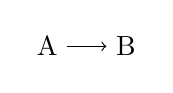
\begin{tikzpicture}
\node (a) at(0,0) {A};
\node (b) at(1,0) {B};
\draw[->] (a) -- (b);
\end{tikzpicture} & Простая п.-с. связь &  \\

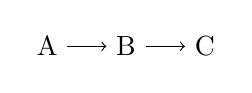
\begin{tikzpicture}
\node (a) at(0,0) {A};
\node (b) at(1,0) {B};
\node (c) at(2,0) {C};
\draw[->] (a) -- (b);
\draw[->] (b) -- (c);
\end{tikzpicture} & Сложная п.-с. связь & \\

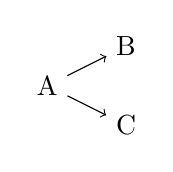
\begin{tikzpicture}
\node (a) at(0,0) {A};
\node (b) at(1,0.5) {B};
\node (c) at(1,-0.5) {C};
\draw[->] (a) -- (b);
\draw[->] (a) -- (c);
\end{tikzpicture} & Общая причина & \\

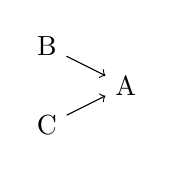
\begin{tikzpicture}
\node (a) at(1,0) {A};
\node (b) at(0,0.5) {B};
\node (c) at(0,-0.5) {C};
\draw[->] (b) -- (a);
\draw[->] (c) -- (a);
\end{tikzpicture} & Множественная причина & \\

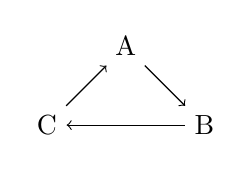
\begin{tikzpicture}
\node (a) at(0,0) {A};
\node (b) at(1,-1) {B};
\node (c) at(-1,-1) {C};
\draw[->] (a) -- (b);
\draw[->] (b) -- (c);
\draw[->] (c) -- (a);

\end{tikzpicture} & Гомеостаз & \\
\end{tabular}
\end{frame}


\section{Ошибки причинно-следственного мышления}

\begin{bframe}

\end{bframe}

\PictureFrame{Correlation}{Корреляция}{\footnotesize Корреляция между возрастом мисс Америки и количеством убийств паром}

\PictureFrame{Correlation1}{Корреляция}{\footnotesize Корреляция между импортом нефти в США и количеством погибших в столкновении с поездами}

%Глава заканчивается почти анекдотическим (но реальным) примером перепутывания причины и следствия аборигенами Новых Гебрид. Они полагали, что наличие вшей ведёт к здоровью. Этот вывод делался на том основании, что больного человека вши покидали (так как вследствие повышенной температуры тела условия существования для них становились некомфортными), тогда как у всех здоровых людей они были (иными словами, наблюдалась положительная корреляция между здоровьем и наличием вшей).

\section{Абдукция}

\begin{bframe}
\begin{center}
\begin{tikzpicture}
\uncover<1->{
\node[align=left] (n)  at (0,0) {
\from{Если идет дождь, земля мокрая}\\
\from{Земля мокрая}\\
\conc{Прошел дождь}
};
}
\uncover<2>{
\draw[color=accent, ultra thick] (n.north west) -- (n.south east);
\draw[color=accent, ultra thick] (n.north east) -- (n.south west);

};

\end{tikzpicture}
\end{center}
\end{bframe}

\begin{bframe}
\begin{Reason}
\from{Наблюдается $B$}
\from{$A$ является причиной $B$}
\from{$A$ {\it наиболее экономное объяснение}}
\conc{$A$ имело место}
\end{Reason}
\end{bframe}

\begin{frame}\frametitle{Критерии объяснения}

\renewcommand{\ReasonWidth}{6cm}

\begin{columns}
\column{0.35\textwidth}
\uncover<1->{Базовые критерии}

\begin{itemize}
\item<2-> Адекватность
\item<3-> Простота
\end{itemize}

\uncover<4->{Дополнительные критерии}
\begin{itemize}
\item<5-> Глубина
\item<7-> Ширина
\item<14-> Фальсифицируемость
\item<24-> Консервативность
\item<26-> Скромность

\end{itemize}

\column{0.65\textwidth}

\only<6>{
\say{Алиса}{Почему ваза разбилась?}
\say{Джон}{Потому что была хрупкая}
}


\from[8-13]{Не включается компьютер}
\from[10-13]{Не работает зарядное устройство}
\from[12-13]{В помещении нет света}
\conc[11-12]{И компьютер, и зарядное устройство сломались}
\conc[9-10]{Компьютер сломался}
\conc[13]{Нет электричества}

\say[15-17]{Алиса}{Что-то я неважно себя чувствую}
\say[16-17]{Урсула}{У вас, наверное, аура потускнела}
\say[17]{Урсула}{Давайте я вам проведу чистку за 100\$...}

\say[18-23]{Джон}{Почему нет воды?}
\say[19-23]{Джеймс}{Рептилоиды опять досаждают! Конечно, это они отключили воду}
\say[20-23]{Джон}{Но я читал в газете, что трубы в нашем городе не ремонтировали уже 30 лет. Может, дело в этом?}
\say[21-23]{Джеймс}{Это ложь. Просто рептилоиды и газеты контролируют...}
\say[22-23]{Джон}{Надо вывести их на чистую воду! Давай всем расскажем об этом!}
\say[23]{Джеймс}{Не выйдет. Тебя упекут в сумасшедший дом, потому что полиция и врачи -- все поголовно рептилоиды}

\from[25]{Я пришел в мой любимый ресторан в 18-00, и он не работает}
\conc[25]{Наверное, теперь этот ресторан будет работать только по утрам}

\from[27-]{Трамвая нет уже 20 минут}
\conc[28]{Наверное, трамваи в городе больше никогда ходить не будут}
\conc[29]{Наверное, трамваи на линии больше никогда ходить не будут}
\conc[30]{Наверное, трамваи на линии некоторое время не ходят}
\conc[31]{Наверное, трамваи на линии некоторое время не ходят из-за аварии}


\end{columns}
\end{frame}

\section{Аналогия}

\begin{bframe}



\end{bframe}


\end{document}